\documentclass[12pt]{article}
\usepackage[margin=2.5cm]{geometry}
\usepackage{enumerate}
\usepackage{amsfonts}
\usepackage{amsmath}
\usepackage{fancyhdr}
\usepackage{amsmath}
\usepackage{amssymb}
\usepackage{amsthm}
\usepackage{mdframed}
\usepackage{graphicx}
\usepackage{subcaption}
\usepackage{adjustbox}
\usepackage{listings}
\usepackage{xcolor}
\usepackage{booktabs}
\usepackage[utf]{kotex}
\usepackage{hyperref}
\usepackage{accents}

\definecolor{codegreen}{rgb}{0,0.6,0}
\definecolor{codegray}{rgb}{0.5,0.5,0.5}
\definecolor{codepurple}{rgb}{0.58,0,0.82}
\definecolor{backcolour}{rgb}{0.95,0.95,0.92}

\lstdefinestyle{mystyle}{
    backgroundcolor=\color{backcolour},
    commentstyle=\color{codegreen},
    keywordstyle=\color{magenta},
    numberstyle=\tiny\color{codegray},
    stringstyle=\color{codepurple},
    basicstyle=\ttfamily\footnotesize,
    breakatwhitespace=false,
    breaklines=true,
    captionpos=b,
    keepspaces=true,
    numbers=left,
    numbersep=5pt,
    showspaces=false,
    showstringspaces=false,
    showtabs=false,
    tabsize=1
}

\lstset{style=mystyle}

\pagestyle{fancy}
\renewcommand{\headrulewidth}{0.4pt}
\lhead{CSC 343}
\rhead{Worksheet 15 (final)}

\begin{document}
\title{CSC343 Worksheet 15 (final)}
\maketitle

\begin{enumerate}[1.]
    \item \textbf{Exercise 4.7.1:} Draw a UML diagram for the problem of Exercise 4.1.1.
    \item \textbf{Exercise 4.7.2:} Modify your diagram from Exercise 4.7.1 in accordance with the requirements of Exercise 4.1.2.
    \item \textbf{Exercise 4.7.3:} Repeat Exercise 4.1.3 using UML.
    \item \textbf{Exercise 4.7.4:} Repeat Exercise 4.1.6 using UML.
    \item \textbf{Exercise 4.7.5:} Repeat Exercise 4.1. 7 using UML. Are your subclasses disjoint or overlapping? Are they complete or partial?
    \item \textbf{Exercise 4.7.6:} Repeat Exercise 4.1.9 using UML.
    \item \textbf{Exercise 4.7.7:} Convert the E/R diagram of Fig. 4.30 to a UML diagram.
    \item \textbf{Exercise 4.7.8:} How would you represent the 3-way relationship of Contracts among movies, stars, and studios (see Fig. 4.4) in UML?

    \begin{center}
    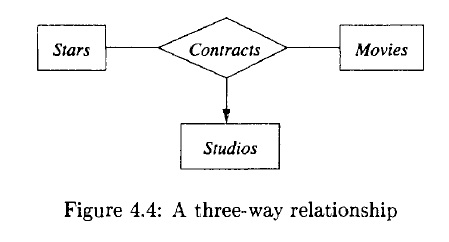
\includegraphics[width=0.6\linewidth]{images/worksheet_15_1.png}
    \end{center}

    \item \textbf{Exercise 4.7.9:} Repeat Exercise 4.2.5 using UML.
    \item \textbf{Exercise 4.8.1:} Convert the UML diagram of Fig. 4.43 to relations.
    \item \textbf{Exercise 4.8.2:} Convert the following UML diagrams to relations:

    \begin{enumerate}[a)]
        \item Figure 4.37.
        \item Figure 4.40.
        \item Your solution to Exercise 4.7.1.
        \item Your solution to Exercise 4.7.3.
        \item Your solution to Exercise 4.7.4.
        \item Your solution to Exercise 4.7.6.
    \end{enumerate}

    \item \textbf{Exercise 4.8.3:} How many relations do we create, using the object-oriented
    approach, if we have a three-level hierarchy with three subclasses of each class
    at the first and second levels, and that hierarchy is:

    \begin{enumerate}[a)]
        \item Disjoint and complete at each level.
        \item Disjoint but not complete at each level.
        \item Neither disjoint nor complete.
    \end{enumerate}
\end{enumerate}

\end{document}